%%%%%%%%%%%%%%%%%%%%%%% file template.tex %%%%%%%%%%%%%%%%%%%%%%%%%
%
% This is a general template file for the LaTeX package SVJour3
% for Springer journals.          Springer Heidelberg 2010/09/16
%
% Copy it to a new file with a new name and use it as the basis
% for your article. Delete % signs as needed.
%
% This template includes a few options for different layouts and
% content for various journals. Please consult a previous issue of
% your journal as needed.
%
%%%%%%%%%%%%%%%%%%%%%%%%%%%%%%%%%%%%%%%%%%%%%%%%%%%%%%%%%%%%%%%%%%%
%
% First comes an example EPS file -- just ignore it and
% proceed on the \documentclass line
% your LaTeX will extract the file if required
\begin{filecontents*}{example.eps}
%!PS-Adobe-3.0 EPSF-3.0
%%BoundingBox: 19 19 221 221
%%CreationDate: Mon Sep 29 1997
%%Creator: programmed by hand (JK)
%%EndComments
gsave
newpath
  20 20 moveto
  20 220 lineto
  220 220 lineto
  220 20 lineto
closepath
2 setlinewidth
gsave
  .4 setgray fill
grestore
stroke
grestore
\end{filecontents*}
%
\RequirePackage{fix-cm}
%
%\documentclass{svjour3}                     % onecolumn (standard format)
%\documentclass[smallcondensed]{svjour3}     % onecolumn (ditto)
\documentclass[smallextended]{svjour3}       % onecolumn (second format)
%\documentclass[twocolumn]{svjour3}          % twocolumn
%
\smartqed  % flush right qed marks, e.g. at end of proof
%
\usepackage{graphicx}
\usepackage{amssymb}
\usepackage{amsmath}
%
% \usepackage{mathptmx}      % use Times fonts if available on your TeX system
%
% insert here the call for the packages your document requires
%\usepackage{latexsym}
% etc.
\usepackage{fixltx2e}
\usepackage[]{algorithm2e}
%
% please place your own definitions here and don't use \def but
% \newcommand{}{}
%
% Insert the name of "your journal" with
% \journalname{myjournal}
%
\begin{document}

\title{A comprehensive performance analysis of various Information Retrieval algorithms for treccar experiments%\thanks{Grants or other notes
%about the article that should go on the front page should be
%placed here. General acknowledgments should be placed at the end of the article.}
}
\subtitle{Internal documentation}

%\titlerunning{Short form of title}        % if too long for running head

\author{Sumanta Kashyapi         \and
        Dr. Laura Dietz %etc.
}

%\authorrunning{Short form of author list} % if too long for running head

\institute{F. Author \at
              first address \\
              Tel.: +123-45-678910\\
              Fax: +123-45-678910\\
              \email{fauthor@example.com}           %  \\
%             \emph{Present address:} of F. Author  %  if needed
           \and
           S. Author \at
              second address
}

\date{Received: date / Accepted: date}
% The correct dates will be entered by the editor


\maketitle

\begin{abstract}
Abstract goes here with purpose, approaches and results.
\keywords{Topic modeling \and LDA \and Information retreival \and KMeans clustering \and Unigram topic model}
% \PACS{PACS code1 \and PACS code2 \and more}
% \subclass{MSC code1 \and MSC code2 \and more}
\end{abstract}

\section{Introduction}
\label{intro}
Categorization of large set of textual materials is a well traversed track of research in the field of information retrieval. Typically in these problems we have a collection of text documents as our input. Using the textual information contained in each document we are to determine to which pre-defined category it belongs. In our case, we have a set of M articles $(A_m \mid m \in \mathbb{N}, m \leq M)$. For each article A\textsubscript{m} we have a set of K\textsubscript{m} section labels 
$(S_{mk} \mid k \in \mathbb{N}, k \leq K_m)$ and a set of N\textsubscript{m} textual content or paragraphs 
$(P_{mn} \mid n \in \mathbb{N}, n \leq N_m)$ relevant to the article. For each article we have to map it's section labels to paragraphs based on the information we extract from the set of paragraphs. The assignment results for all the articles are compared with the correct assignment provided in a ground truth file.
An evaluation framework is developed to quantify this comparison which in turn can be utilized to determine which categorization are better than the rest.
Various categorization and classification algorithms can be used for the assignment task and for each approach we can measure it's effectiveness using the evaluation framework. For the experiments described here, we have used LDA topic modeling, KMeans, Unigram topic modeling and some of their variations. Our aim will be to identify which components of these algorithms are responsible for good results from the performance measures calculated by our evaluation framework. We will also carry out a feasibility study of a hybrid approach consisting of the best components for this task.


\section{LDA topic modeling}
\label{sec:lda}
LDA theory and mallet implementation details goes here.
\paragraph{Implementation} mallet implementation details.
\section{KMeans algorithm}
\label{sec:kmeans}
KMeans theory and mallet implementation details goes here.
\paragraph{Implementation} mallet implementation details.
\section{Unigram topic model}
\label{sec:umm}
In his paper, author Blei describes how his LDA model extended from the simple Unigram mixture model. According to the unigram mixture model the probability of a document $p(\mathbf{w})$ in a corpus can be expressed as:
$$ p(\mathbf{w}) = \sum_z p(z) \prod_{n=1}^N p(w_n \mid z)$$
However, in this paper we considered modifying the existing LDA implementation to have an additional constraint that will enforce unigram behaviour to typical LDA model. The constraint we tried to implement here is each token in a single document has to agree upon a single topic in a single iteration. So we simply would not allow a state during any itrerations in which some token is assigned a topic different than it's adjacent ones. We did this by assigning topics to an entire document rather than individual tokens. However, we still considered individual tokens for probability calculations of the next topic assignment.
\begin{algorithm}[htp]
 \KwData{Pre-processed corpus}
 \KwResult{Trained Unigram topic model for input corpus}
 \For{each doc $ m $ in corpus where $ m \in [1,M] $}{
  \For{each topic i=1 to k}{
   calculate $ p'(m_i \mid \overrightarrow{m_{-i}}, \overrightarrow{w})$\;
  }
  sample a new topic $ \widetilde{k} \sim p'(m) $\;
  \For{each token $ t \in [1, T_m] $ in doc $ m $}{
   decrement count from all data structures involving old topic assignment\;
   assign new topic $ \widetilde{k} $ to all data structures\;
  }
 }
 \caption{Unigram topic model training phase}
\end{algorithm}
Calculation of the distribution $ p'(m)$, from where $ \widetilde{k}$ is drawn, dominates the training phase. According to unigram model a topic is assigned to a whole document m and therefore all tokens t = 1 to $ T_m$ inside that document m takes the same topic $ \widetilde{k}$ or $ z_t = \widetilde{k}$ for all t = 1 to $ T_m$. Hence each probability in the distribution $ p'(m)$ can be expressed as:
$$ p'(m_i \mid \overrightarrow{m_{-i}}, \overrightarrow{w}) =
   \prod_{t=1}^{T_m} p_t(z_t = k \mid \overrightarrow{z_{-t}}, \overrightarrow{w}) $$

Being an extension of original LDA algorithm, we can still use the proportional relation
$$ p_t(z_t = k \mid \overrightarrow{z_{-t}}, \overrightarrow{w}) \propto 
   \frac{n_{k,-t}^{(v)}+\beta_v}{\sum_{v=1}^V (n_{k,-t}^{(v)}+\beta_v)}(n_{m,-t}^{(k)}+\alpha_k)
$$
But $ n_{m,-t}^{(k)} = 0$ for all m and k, so our proportional equation simplifies to:

\begin{align*}
p'(m_i \mid \overrightarrow{m_{-i}}, \overrightarrow{w}) & \propto
   \prod_{t=1}^{T_m} \frac{n_{k,-t}^{(v)}+\beta_v}{\sum_{v=1}^V (n_{k,-t}^{(v)}+\beta_v)} \\
   & \parbox{20em}{ignoring proportionality constant and assuming symmetrical $ \beta$ distribution over vocabulary} \\
   &= \prod_{t=1}^{T_m} \frac{n_{k,-t}^{(v)}+\beta}{\sum_{v=1}^V n_{k,-t}^{(v)}+\beta Sum}  \\
   &= \exp \Bigg[ \sum_{t=1}^{T_m} \log \bigg( n_{k,-t}^{(v)}+\beta \bigg)-T_m \dot{\log \bigg( \sum_{v=1}^V n_{k,-t}^{(v)}+\beta Sum \bigg)} \Bigg] \\
   & \text{in log space}
\end{align*}

While implementing unigram model we computed $ p'(m_i)$ in log space to avoid underflows. Also instead of directly sampling from $ p'$, we used the smoothed version (Jelinek-Mercer smoothing) $ p''$ which is calculated as:
$$ p''(m_i) = \lambda p'(m_i) + (1- \lambda) $$
Here $ \lambda$ is inverse temperature which controls randomness during sampling. In other words, low $ \lambda$ leads to more \textit{exploration} from wide range of topics and high $ \lambda$ will \textit{exploit} from narrow range of topics. The topic inferencer for unigram model, which is used during the section to paragraph assignment, performs similar calculations except, instead of paragraphs in corpus it takes the text content related to section headings.
\paragraph{Implementaion} implementation details.
\section{Evaluation Framework}
\label{sec:3}
Before we try to experiment with different combinations of topic modeling and clustering modules with our treccar corpus, we must have a reliable framework to compare our results. A robust evaluation framework for our experiments is a key element which will help us to be confident about our findings. We will evaluate two aspects of our results. First, we have a set of measures which will determine the accuracy of the clustering that we have done with our set of data elements, which is in this case a set of paragraph objects identified by unique paragraph ids. Note that while measuring how good our clusters are compared to that of the ground truth, we do not utilize the assignment mappings or more precisely the section objects under which each cluster is mapped. In our second set of measure we do just that by comparing our section to paragraph mappings with that of ground truth. 
\subsection{Clustering measures}
\label{sec:4}
In our current evaluation framework we are using two basic statistical measures for evaluating our clustering results.
\subsubsection{Adjusted RAND index}
\label{sec:5}
RAND index is a popular statistical measure used to quantify the similarity between two clusterings done on the same dataset. In our case those two clusterings are resulting clusters from our designed model and the clusters made according to the ground truth file. Although RAND index is often associated with the accuracy of the results but in our case we are using it without the class labels. Typically RAND index,R is calculated as:
\begin{equation}
R = \frac{a+b}{a+b+c+d} = \frac{a+b}{{{n}\choose{2}}} 
\end{equation}
\\where $a,b = $ pairs of paragraphs present in either same or differnt cluster for both clustering,
\\$c,d = $ pairs of paragraphs present in same cluster in one but in differnt cluster in other,
\\$n = $ no. of paragraphs
But this simple RAND index expects the two partitions to have same number of clusters. However, we want the framework to be robust enough so that we can compare our results even when our resulting partition is of different size from that of the ground truth. Hence adjusted RAND index or ARI is used which is calculated as:
\begin{equation}
ARI = \frac{\sum_{ij}{{n_{ij}}\choose{2}}-[\sum_{i}{a_{i}\choose{2}}\sum_{j}{b_{j}\choose{2}}]/{{n}\choose{2}}}{1/2[\sum_{i}{a_{i}\choose{2}}+\sum_{j}{b_{j}\choose{2}}]-[\sum_{i}{a_{i}\choose{2}}\sum_{j}{b_{j}\choose{2}}]/{{n}\choose{2}}}
\end{equation}
\\where $n_{ij}=$ contingency table values from $i$th row and $j$th column
\\$a_{i}=$ contingency table $i$th row sum
\\$b_{j}=$ contingency table $j$th column sum
\subsubsection{Purity}
Purity theory goes here
\subsection{Assignment measures}
\label{sec:6}
After we finish clustering the paragraphs and assign them with their respective cluster labels, we have to assign them to sections. The quality of the section to paragraph assignment is measured using an existing framework, TREC eval, which is designed specifically for this set of problems where we have to evaluate rankings of retrieved information.
\paragraph{Different measures of TREC eval} theory and usage of numq measures, map and rprec with background of precision

\section{Implementation details}
\label{sec:implementation}
The algorithms, models and evaluation framework are developed in java. Mallet API has been used for basic text retrieval tasks and as a starting point for developing all the models used in the experiments.
\subsection{Important classes}
\paragraph{RunExperiment: }
It is the starting point of the evaluation framework. It contains most of the variables that control the workflow of the experiment including which algorithm and which version of it is to be used. It takes all the values for one set of experiments and constructs the topmost loop that calls the appropriate algorithm with it's respective values. Details of the varibles are in Table

\begin{table}
% table caption is above the table
\caption{RunExperiment variables}
\label{tab:iter}       % Give a unique label
% For LaTeX tables use
\begin{tabular}{l|p{60mm}}
\hline\noalign{\smallskip}
Variable & Purpose  \\
\noalign{\smallskip}\hline\noalign{\smallskip}
\textbf{SAVE\_RESULT} & Whether we want to save our results \\
\hline
\textbf{RUN\_BY\_PAGE} & Whether we want to run by page or take the whole corpus as a single page. In case it is false, the problem changes from section to paragraph assignment to page to paragraph assignment. In other words, instead of calculating measures for each page, we now replace all the section titles with page titles and we try to assign paragraphs to it's respective pages. Consequently we calculate a single measure for the entire corpus. \\
\hline
\textbf{CLUSTERING\_MEASURE\_FILENAME} & The name of the file which will store the clustering measures. \\
\hline
\textbf{TRECEVAL\_ASSIGN\_FILENAME} & The name of the file which will store the section to paragraph assignments in trec\_eval format which will be the input for trec\_eval script. \\
\hline
\textbf{SMOOTHED\_UMM} & Whether we are using smoothing in Unigram topic model. \\
\hline
\textbf{model} & Which algorithm/model is to be used. Currently we have five valid strings for this: $ 1=LDA, 2=KMeans, 3=Unigram, 98=Correct, 99=Random $ \\
\hline
\textbf{[meta][Param]} & These are the parameters for algorithms that we can vary. There are currently four parameters available which are $ k$ value, number of iterations for a single call to the respective algorithm, $ \alpha Sum$ and $ \beta Sum$ two hyperparameters for topic modeling. Also for each parameter, we have three bounding values $[meta]$ to calculate different values of the parameter thoroughout the iterations which are start, stop and step. For a particular parameter, we start off the iterations with start value of the parameter until we get to the stop value adding the step value to the current value after each iteration. \\
\hline
\textbf{isVar} & Each boolean value in this array represents one variable. Currently it is of size four and from 0 to 3 it represents $ k, iterations, \alpha Sum and \beta Sum$ respectively. For example, if we have the array as $ [true, false, false, true]$ then it means we will consider $ stop and step$ values of $ k and \beta Sum$ and iterate through different values of $ k and \beta Sum$. \\
\noalign{\smallskip}\hline
\end{tabular}
\end{table}
\paragraph{SingleRun: }
At each iteration of $RunExperiment$, $SingleRun$ is called with appropriate arguments. This is the class which decides which version of which algorithm is to be called. Depending on the $RUN\_BY\_PAGE$ varibale of $RunExperiment$ class, $runExperiment()$ or $runExperimentWholeCorpus()$ method of $SingleRun$ is called from $RunExperiment$. Some important method details are discussed in Table.
\begin{table}
% table caption is above the table
\caption{Important SingleRun methods}
\label{tab:iter}       % Give a unique label
% For LaTeX tables use
\begin{tabular}{l|p{60mm}}
\hline\noalign{\smallskip}
Method & Purpose  \\
\noalign{\smallskip}\hline\noalign{\smallskip}
\textbf{runExperiment} & Performs experiment on per page basis. This method is implemented using algorithm \ref{algo:runExperiment}. \\
\hline
\textbf{runExperimentWholeCorpus} & Performs experiment on the whole corpus. \\
\hline
\textbf{modelAndAssign} & Based on the $model$ parameter passed from $RunExperiment$ different algorithms are called. This method is based on algorithm \ref{algo:modelAndAssign}. \\
\hline
\textbf{convInsAssignToIDAssign} & Coverts mappings from Section Instance object to list of Paragraph instances to mappings from Section id to list of Paragraph ids. \\
\hline
\textbf{assignUsing[algo]} & These methods takes the clusters of paragraphs generated by some algorithm and assigns them to section instances using $[algo]$ algorithm ( $assignUsingKMeans$ uses KMeans). Ideally any changes made to these methods will not affect the results of clustering measures because section to paragraph assignment information is not utilized while calculating those measures. Algorithm \ref{algo:assignUsing} is implemented in this method. \\
\hline
\textbf{matrixAssignment} & This is called from $assignUsing[algo]$ to do the assignment using the KL divergence matrix (for topic modeling algorithms) or the distance matrix (for clustering algorithms). \\
\noalign{\smallskip}\hline
\end{tabular}
\end{table}

\begin{algorithm}[htp]
\label{algo:runExperiment}
 \KwData{Pre-processed corpus and necessary parameters}
 \KwResult{Performance results for each page}
 \For{each page $ p $ in corpus where $ i \in [1,P] $}{
  get Instance Lists of paragraphs and queries for $p$; \\
  call $modelAndAssign()$ to get cluster and assignment results for $p$; \\
  check for any duplicate paragraph assigned; \\
  store results as $p \rightarrow results$; \\
 }
 call $MeasureExperiment$ methods with all $p \rightarrow results$ to obtain performance measures for each $p$; \\
 \If{$SAVE$}{
  save measures to output file \\
 }
 \caption{$runExperiment()$ algorithm}
\end{algorithm}

\begin{algorithm}[htp]
\label{algo:modelAndAssign}
 \SetAlgoLined\DontPrintSemicolon
 \SetKwFunction{modelAndAssign}{modelAssign}\SetKwFunction{getNumTopics}{getNumTopics}
 \SetKwProg{myalg}{Algorithm}{}{}
 \myalg{\modelAndAssign{}}{
  \Switch{$model$}{
   \Case{1}{
    \getNumTopics{}\; 
    train LDA model with $numTopics, \alpha Sum, \beta Sum, $ list of paragraph elements; \\
    call $assignUsingLDA()$; \\
   } 
   \Case{2}{
    \getNumTopics{}\;
    train KMeans model with $numTopics, $ list of paragraph elements; \\
    call $assignUsingKMeans()$; \\
   }
   \Case{3}{
    \getNumTopics{}\;
    train UMM model with $numTopics, \beta Sum, $ list of paragraph elements; \\
    call $assignUsingUMM()$; \\
   }
   \Case{98}{
    call $assignUsingAllCorrect()$; \tcp*{baseline measures}
   }
   \Case{99}{
    call $assignUsingRandom()$; \tcp*{baseline measures}
   }
  }
 }{}
 \setcounter{AlgoLine}{0}
 \SetKwProg{myproc}{Procedure}{}{}
 \myproc{\getNumTopics{}}{
  \If{$k==0$}{
   $numTopics =$ size of query list; \\
  }
  \Else{
   \If{$k \geq size of paragraph list$}{
    $numTopics =$ size of paragraph list; \\
   }
   \Else{
    $numTopics = k$
   }
  }  
 }
 \caption{$modelAndAssign()$ algorithm}
\end{algorithm}

\begin{algorithm}[htp]
\label{algo:assignUsing}
 \SetAlgoLined\DontPrintSemicolon
 \ForEach{paragraph $p$ in list of paragraphs}{
  \ForEach{query $q$ in list of queries}{
  calculate $paraQueryMatrix[p][q] = assignVal$ for $p$ and $q$\; \tcc{$assignVal$ is the KL-div value for topic modeling algorithms and metric distance for clustering algorithms so that the value becomes proportional to the quality of $p$ to $q$ assignment}
  }
 }
 initialize $isParaAssigned[] = false$\;
 \ForEach{paragraph $p$ in list of paragraphs}{
  $bestQueryForPara = q$ where $paraQueryMatrix[p][q] = \min{paraQueryMatrix[p]}$\;
 }
 \While{$checkIfDone()$}{ \tcc{$checkIfDone()$ will return true when all values in $paraQueryMatrix$ is 0}
  get index $(p,q)$ of minimum positive value in $paraQueryMatrix$\;
  assign $para[p] \rightarrow query[q]$\;
  put $-1$ in place of row $p$ and column $q$ of $paraQueryMatrix$\;
  $isParaAssigned[p] = true$\;
 }
 \ForEach{paragraph $p$ in list of paragraphs}{
  \If{$isParaAssigned[p] = false$}{
   assign $para[p] \rightarrow bestQueryForPara[q]$\;
  }
 }
 \caption{$assignUsing[modelName]()$ algorithm}
\end{algorithm}

\begin{algorithm}[htp]
\label{algo:contMat}
 \SetAlgoLined\DontPrintSemicolon
 \ForEach{page $pg$ in corpus}{
  obtain clusters from $ResultForPage[pg]$\;
 }
 \ForEach{$key$ in $gtMap$}{ \tcc{$gtMap$ is the mapping between pageID and paragraph clusters according to ground truth file}
  \If{WHOLE\_CORPUS\_MODE}{
   get the list of lists of paragraphs as $gtClusters$\;
  }
  \ElseIf{$key$ starts with pageID}{
   add $gtMap[key]$ to $gtClusters$\;
  }
  $candClusters = clusters[pg]$\;
  intialize $contMat[gtClusters[pg].size()][candClusters.size()]$\; \tcp*{Contingency Matrix}
  \ForEach{row $r$ in $contMat$}{
   \ForEach{column $c$ in $contMat$}{
    $correct = gtClusters[r]$\;
    $candidate = candClusters[c]$\;
    $match = $no. of matches between $correct$ and $candidate$\;
    $contMat[r][c] = match$\;
   }
  }
 }
 \caption{Algorithm to form contingency matrix}
\end{algorithm}  
\paragraph{ResultForPage: }
This class is generated for each page and holds the clusters of paragraph ids ($paraClusters$) and the mapping of section ids to list of paragraph ids ($queryParaAssignment$).
\paragraph{MeasureExperiment: }
This class calculates the cluatering measures for a single page. Currently it calculates two measures, adjusted RAND index ($calculateRANDPerPage$) and Purity ($calculatePurityPerPage$) from the contingency matrix formed using the algorithm \ref{algo:contMat}. Later on in $SingleRun$ these values are used to get the mean and standard error for the current experiment.

\subsection{Sequence of execution}

\section{Experimental results}
\label{sec:results}
\subsection{Baseline experiments} Two sets of experiments are carried out to form a baseline for other algorithms. In first set, we randomly assigned paragraphs to sections for each article. For this random assignment we got mean RAND index to be 0.0032. When it is ensured that every section got at least one paragraph, it comes down to -0.0014. more to add here purity, map, rprec
\begin{figure}
    \centering
    \begin{minipage}{0.45\textwidth}
        \centering
        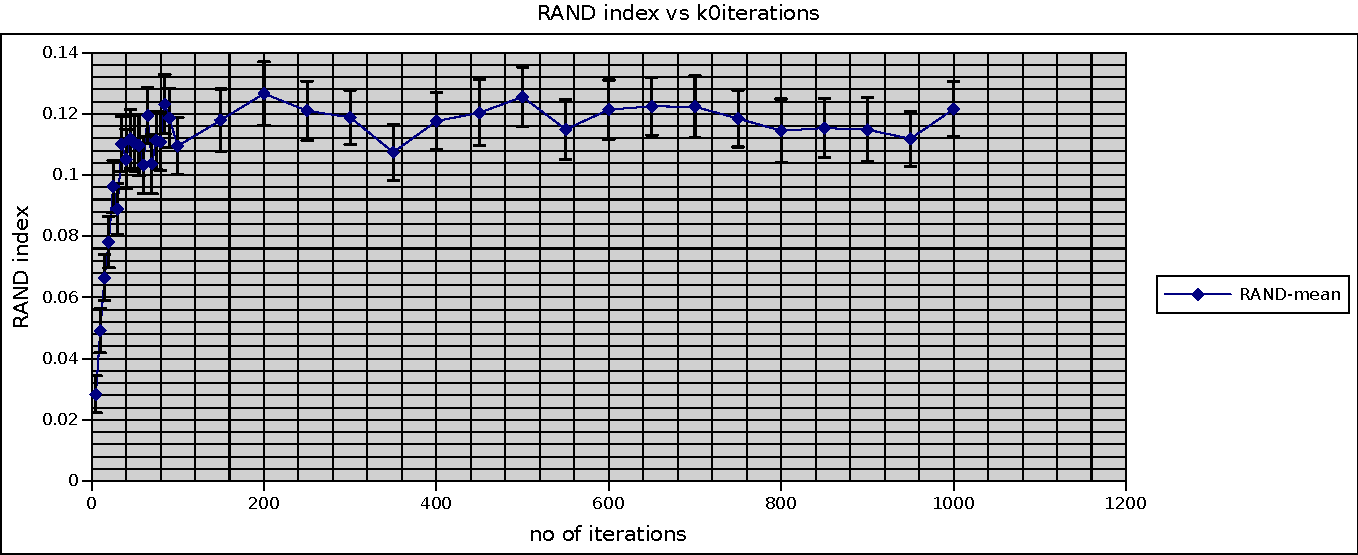
\includegraphics[width=0.9\textwidth]{rand_k0iter_lda.pdf}
        \caption{Minimum no. of iterations of LDA topic modeling for RAND}
    \end{minipage}\hfill
    \begin{minipage}{0.45\textwidth}
        \centering
        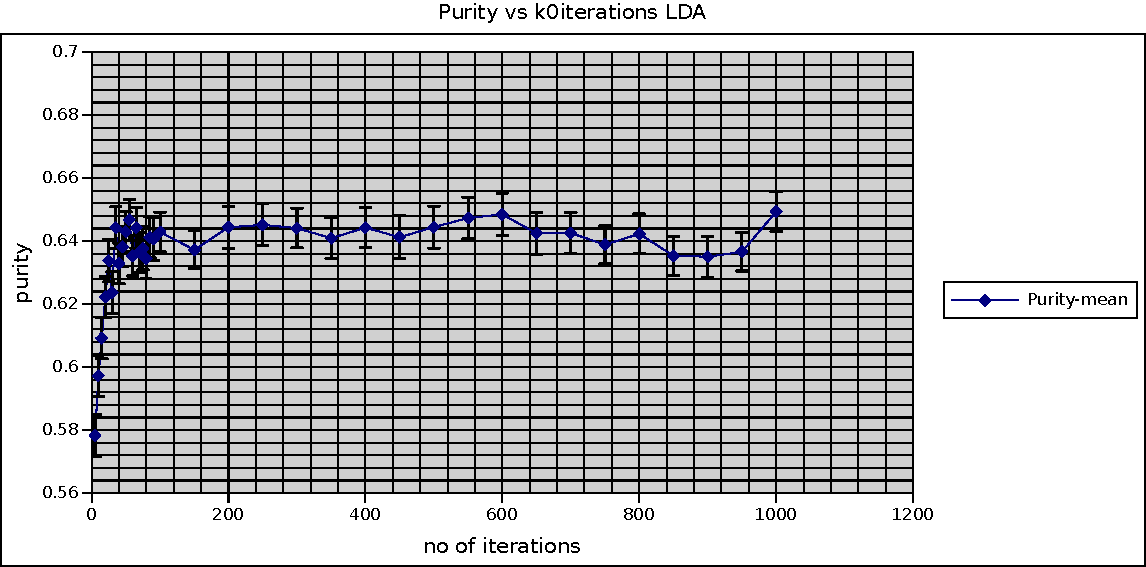
\includegraphics[width=0.9\textwidth]{purity_k0iter_lda.pdf}
        \caption{Minimum no. of iterations of LDA topic modeling for Purity}
    \end{minipage}
\end{figure}
\begin{figure}
    \centering
    \begin{minipage}{0.45\textwidth}
        \centering
        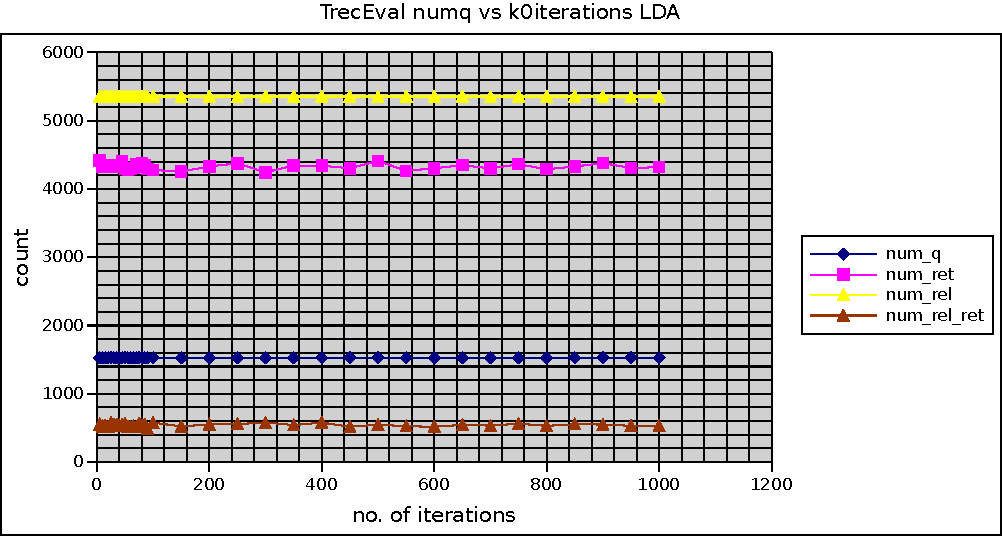
\includegraphics[width=0.9\textwidth]{numq_k0iter_lda.pdf}
        \caption{Minimum no. of iterations of LDA topic modeling for numq measures}
    \end{minipage}\hfill
    \begin{minipage}{0.45\textwidth}
        \centering
        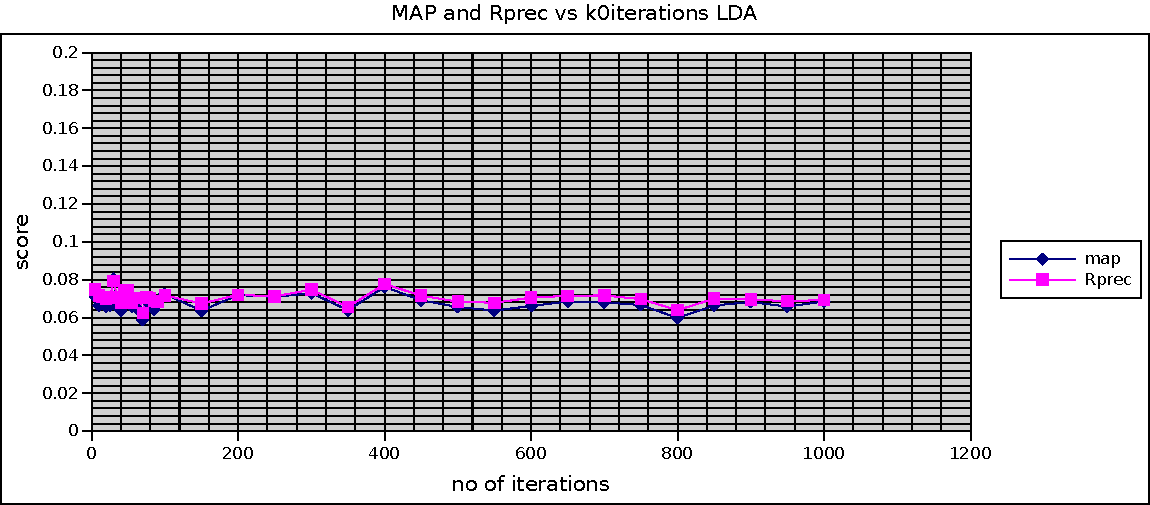
\includegraphics[width=0.9\textwidth]{map_rprec_k0iter_lda.pdf}
        \caption{Minimum no. of iterations of LDA topic modeling for MAP and Rprec}
    \end{minipage}
\end{figure}
\subsection{Minimum no. of iterations} Three sets of experiments were carried out for each algorithm to get the minimum number of iterations needed of the respective algorithm to reach sufficiently close to the highest result it can achieve. Each set of experiments were done using 4 set of measures; Adjusted RAND index, Purity, four numq measures from trec\_eval tool and precision measures. The plots of this study for LDA algorithm are shown in figures 3 to 6 and for Unigram topic model algorithm are shown in figures 7 to 10. Iteresting point to note here is that for Unigram topic modeling none of the measures seems to be affected by number of iterations. Obtained results are presented in Table 1.
% For tables use
\begin{table}
% table caption is above the table
\caption{Minimum no. of iterations}
\label{tab:iter}       % Give a unique label
% For LaTeX tables use
\begin{tabular}{lllllll}
\hline\noalign{\smallskip}
Algorithm & min. iterations for RAND & purity & numq measures & MAP & Rprec & chosen iteration  \\
\noalign{\smallskip}\hline\noalign{\smallskip}
LDA & $ >80$ & $ >40$ & NE & NE & NE & 100 \\
Unigram & NE & NE & NE & NE & NE & 100 \\
\noalign{\smallskip}\hline
NE = No Effect
\end{tabular}
\end{table}

\begin{figure}
    \centering
    \begin{minipage}{0.45\textwidth}
        \centering
        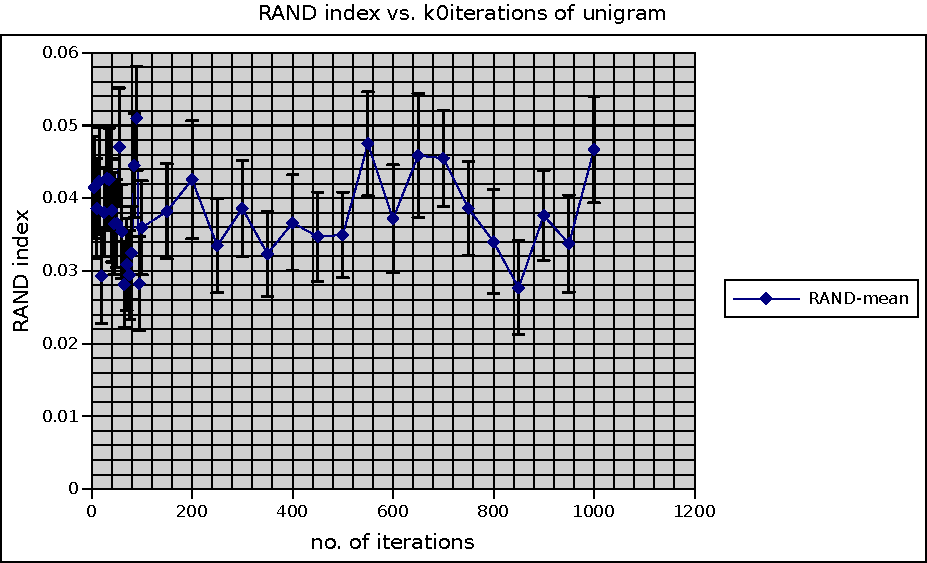
\includegraphics[width=0.9\textwidth]{rand_k0iter_umm.pdf}
        \caption{Minimum no. of iterations of Unigram topic modeling for RAND}
    \end{minipage}\hfill
    \begin{minipage}{0.45\textwidth}
        \centering
        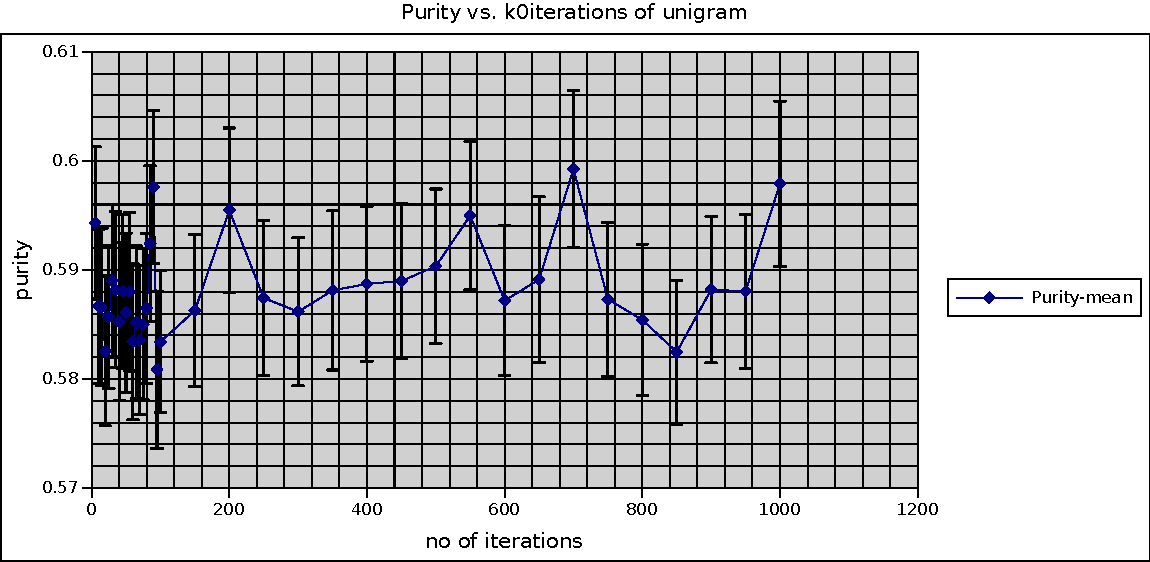
\includegraphics[width=0.9\textwidth]{purity_k0iter_umm.pdf}
        \caption{Minimum no. of iterations of Unigram topic modeling for Purity}
    \end{minipage}
\end{figure}
\begin{figure}
    \centering
    \begin{minipage}{0.45\textwidth}
        \centering
        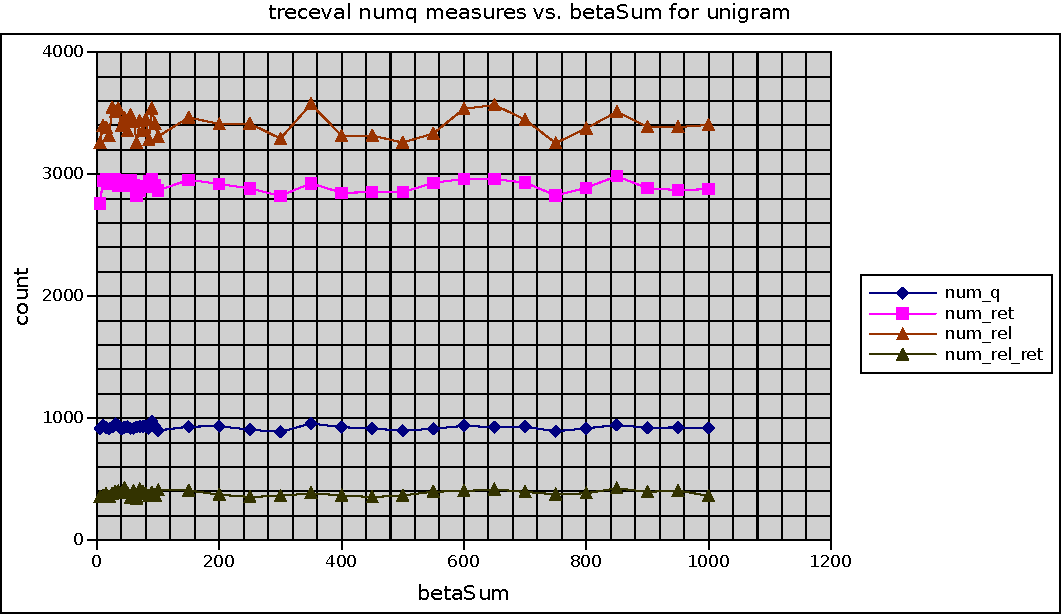
\includegraphics[width=0.9\textwidth]{numq_k0iter_umm.pdf}
        \caption{Minimum no. of iterations of Unigram topic modeling for numq measures}
    \end{minipage}\hfill
    \begin{minipage}{0.45\textwidth}
        \centering
        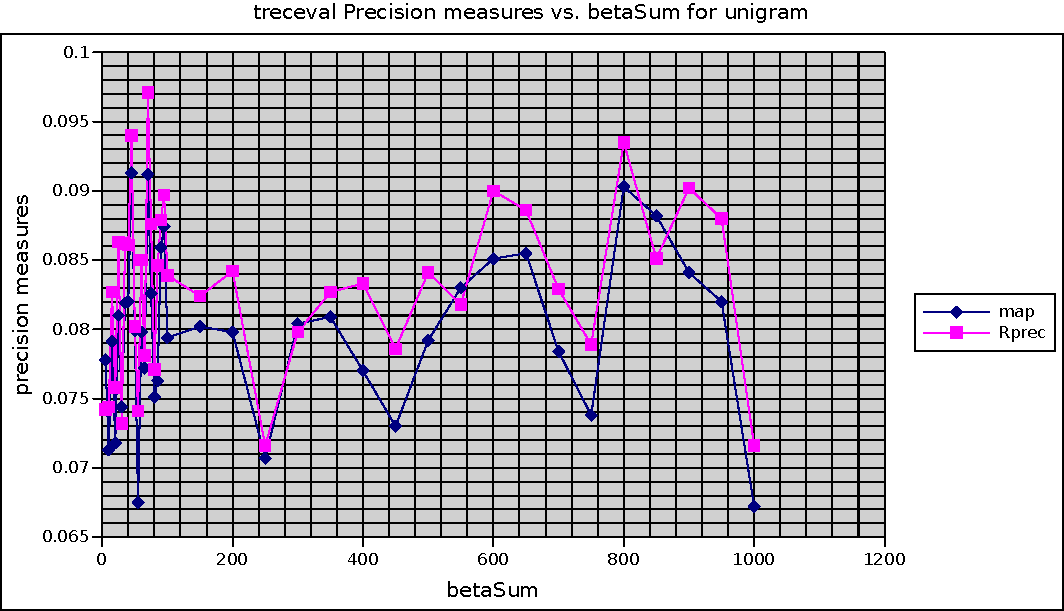
\includegraphics[width=0.9\textwidth]{prec_k0iter_umm.pdf}
        \caption{Minimum no. of iterations of Unigram topic modeling for MAP and Rprec}
    \end{minipage}
\end{figure}

\subsection{Hyper parameter learning} LDA algorithm has two hyperparameters, $ \alpha$ and $ \beta$. We have to learn the optimum value for both of these parameters for our particular corpus using the evaluation framework. Also for Unigram topic modeling algorithm we have the smoothing factor (inverse temperature) $ \lambda$. To get the optimum values of these variables we run the algorithm over a sufficiently large range of a parameter while keeping rest at a constant value. Then we measure various evaluation metrics and find out a narrow range of parameter values for which we are getting sufficiently good measures. 
\paragraph{Optimum alphaSum and betaSum for LDA}Figures from 9 to 12 plots result obtained from the experiments to learn optimum alphaSum and betaSum for LDA algorithm. From these charts we found optimum range for alphaSum to be 0.8 to 1.2 and optimum range for betaSum to be 100 to 300. For subsequent experiments with LDA algorithm, we chose alphaSum and betaSum values to be 1.0 and 260.
\paragraph{Optimum lambda and betaSum for Unigram topic model}
\begin{figure}
    \centering
    \begin{minipage}{0.45\textwidth}
        \centering
        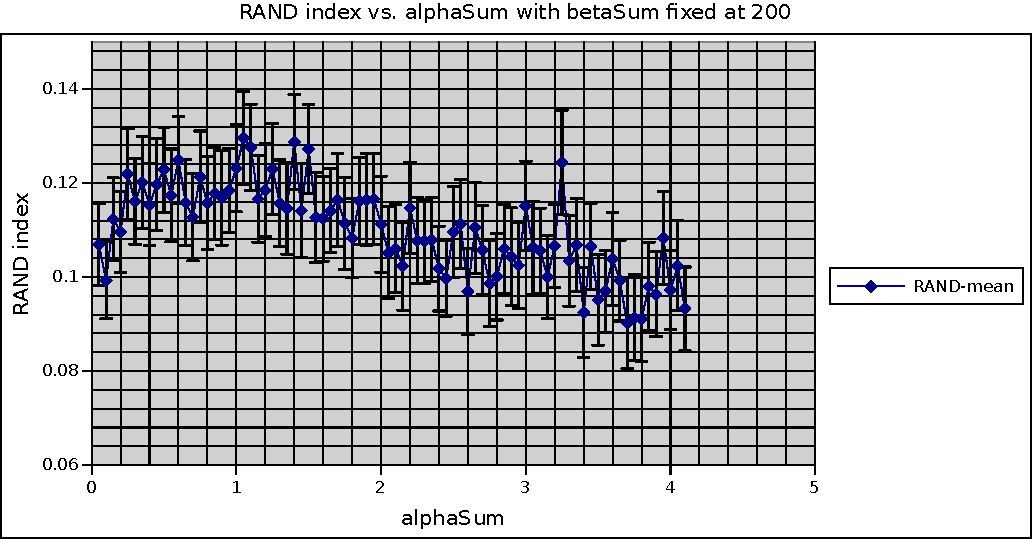
\includegraphics[width=0.9\textwidth]{alphaSum_rand_lda.pdf}
        \caption{Learning optimum alphaSum of LDA for RAND with betaSum, iterations fixed}
    \end{minipage}\hfill
    \begin{minipage}{0.45\textwidth}
        \centering
        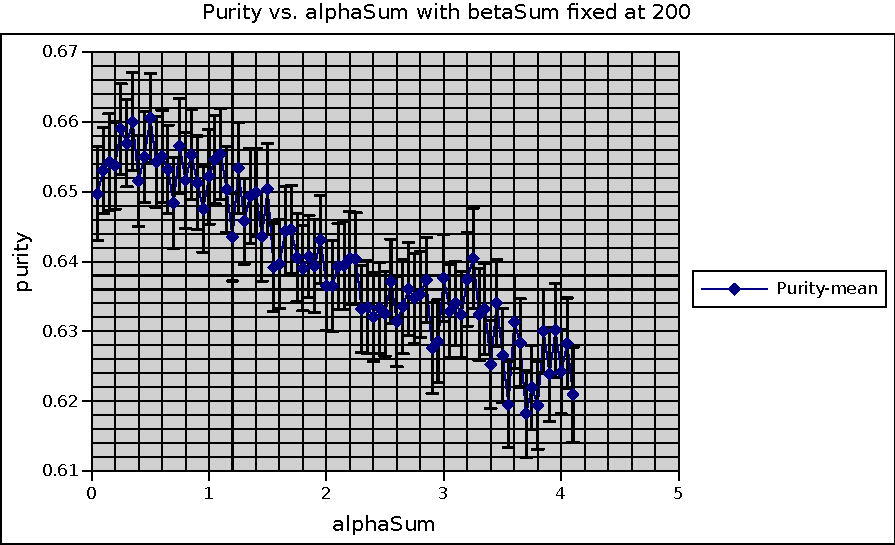
\includegraphics[width=0.9\textwidth]{alphaSum_purity_lda.pdf}
        \caption{Learning optimum alphaSum of LDA for Purity with betaSum, iterations fixed}
    \end{minipage}
\end{figure}
\begin{figure}
    \centering
    \begin{minipage}{0.45\textwidth}
        \centering
        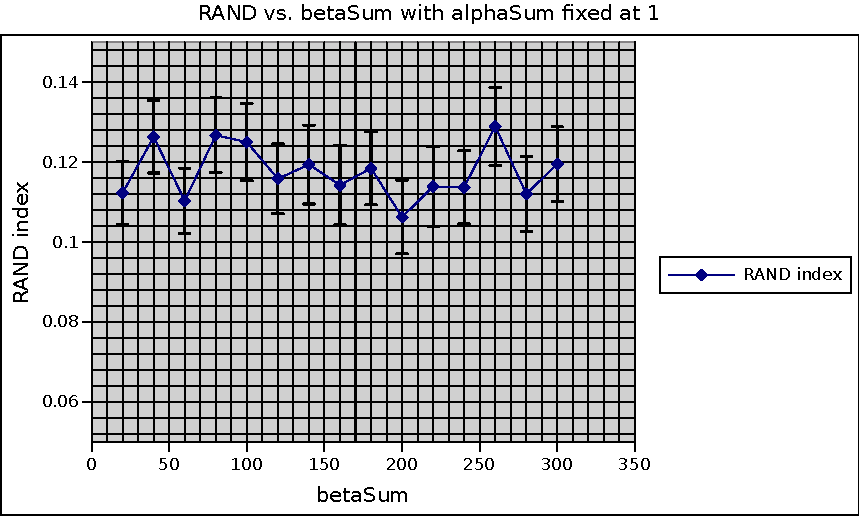
\includegraphics[width=0.9\textwidth]{betaSum_rand_lda.pdf}
        \caption{Learning optimum betaSum of LDA for RAND with alphaSum, iterations fixed}
    \end{minipage}\hfill
    \begin{minipage}{0.45\textwidth}
        \centering
        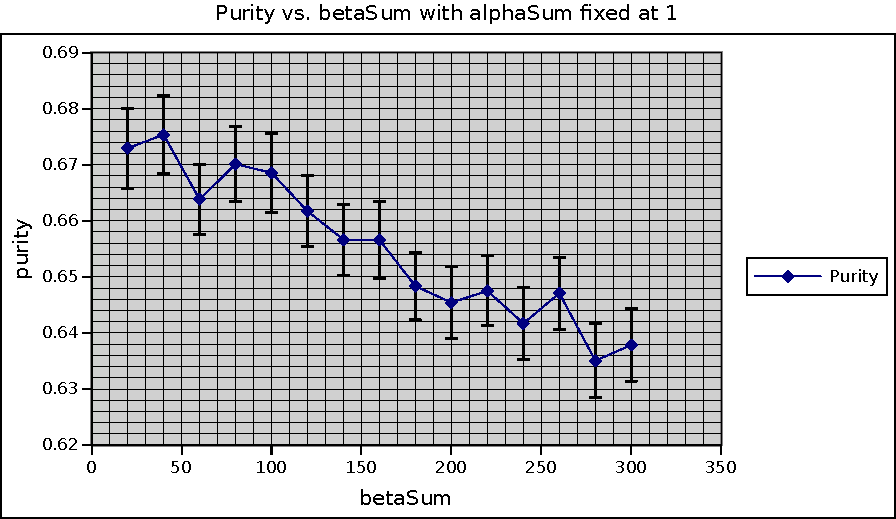
\includegraphics[width=0.9\textwidth]{betaSum_purity_lda.pdf}
        \caption{Learning optimum betaSum of LDA for Purity with alphaSum, iterations fixed}
    \end{minipage}
\end{figure}
\subsection{KMeans clustering results} plots go here
\subsection{Comparison of results with true no. of sections and k} After we have decided the optimum values of hyperparameters for all the algorithms, we compare the measures from different algorithms by varying $k$ and also at $k = $true no. of sections. This will give us an idea about the effectiveness of each algorithm for the task.

\begin{figure}
    \centering
    \begin{minipage}{0.45\textwidth}
        \centering
        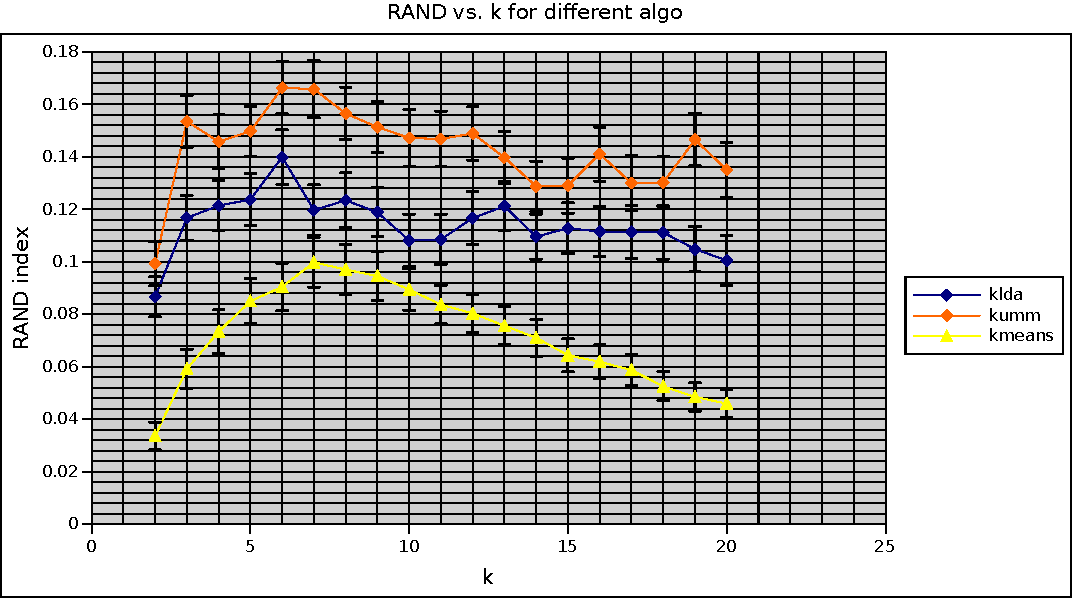
\includegraphics[width=0.9\textwidth]{rand_comp.pdf}
        \caption{Comparison of RAND index vs. k}
    \end{minipage}\hfill
    \begin{minipage}{0.45\textwidth}
        \centering
        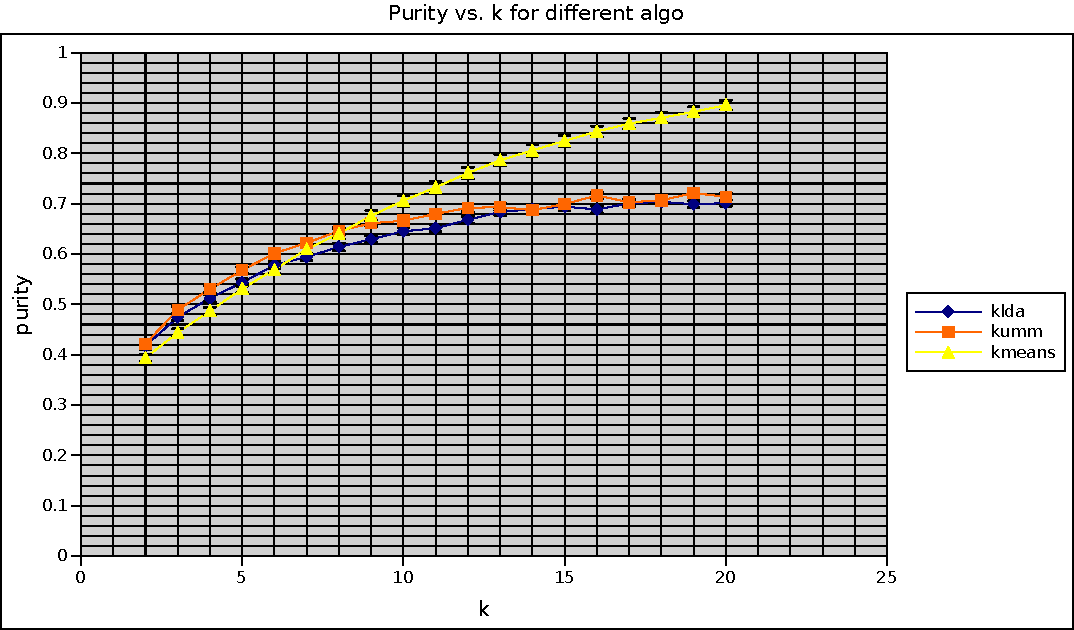
\includegraphics[width=0.9\textwidth]{purity_comp.pdf}
        \caption{Comparison of purity vs. k}
    \end{minipage}
\end{figure}
\begin{figure}
    \centering
    \begin{minipage}{0.45\textwidth}
        \centering
        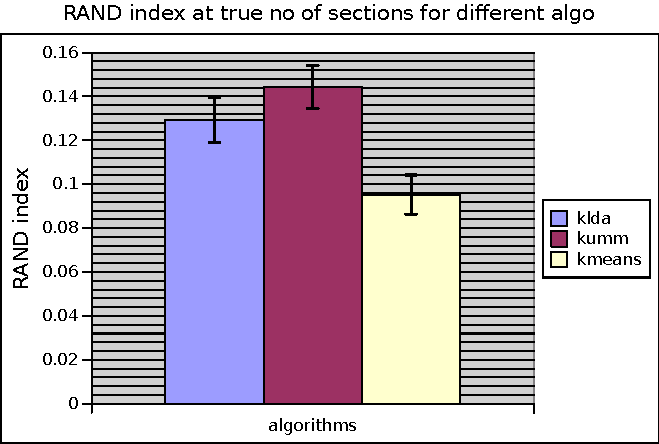
\includegraphics[width=0.9\textwidth]{rand_k0_comp.pdf}
        \caption{Comparison of RAND index at true no. of sections}
    \end{minipage}\hfill
    \begin{minipage}{0.45\textwidth}
        \centering
        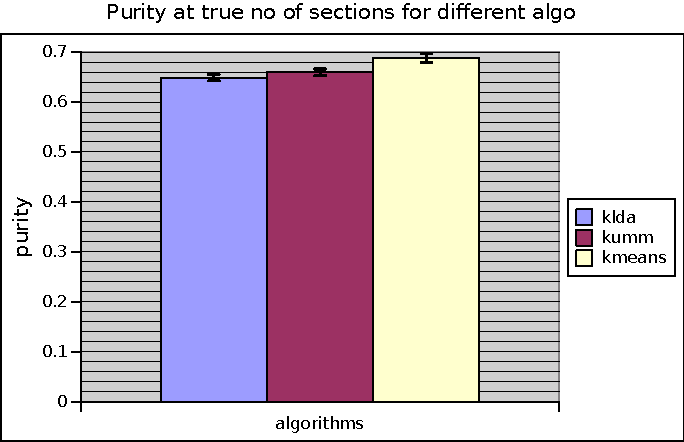
\includegraphics[width=0.9\textwidth]{purity_k0_comp.pdf}
        \caption{Comparison of RAND index at true no. of sections}
    \end{minipage}
\end{figure}

\subsection{Comparison of results with variations of algo} plots go here
\subsection{Results in whole corpus mode} plots go here
\subsection{Difficulty analysis of the corpus} plots go here
%\begin{acknowledgements}
%If you'd like to thank anyone, place your comments here
%and remove the percent signs.
%\end{acknowledgements}

% BibTeX users please use one of
%\bibliographystyle{spbasic}      % basic style, author-year citations
%\bibliographystyle{spmpsci}      % mathematics and physical sciences
%\bibliographystyle{spphys}       % APS-like style for physics
%\bibliography{}   % name your BibTeX data base

% Non-BibTeX users please use
\begin{thebibliography}{}
%
% and use \bibitem to create references. Consult the Instructions
% for authors for reference list style.
%
\bibitem{RefJ}
% Format for Journal Reference
Author, Article title, Journal, Volume, page numbers (year)
% Format for books
\bibitem{RefB}
Author, Book title, page numbers. Publisher, place (year)
% etc
\end{thebibliography}

\end{document}
% end of file template.tex

